% Foliensatz: "AFu-Kurs nach DJ4UF" von DK0TU, Amateurfunkgruppe der TU Berlin
% Lizenz: CC BY-NC-SA 3.0 de (http://creativecommons.org/licenses/by-nc-sa/3.0/de/)
% Autoren:Felix Baum <baum@campus.tu-berlin.de>, Martin Deutschmann,

\documentclass[aspectratio=169]{beamer}

\usepackage[ngerman]{babel} % deutsche Worttrennung etc.
\usepackage[utf8]{inputenc} % UTF8 Text

\usepackage[super, comma, numbers, square, sort]{natbib}

\usepackage{hyperref}       % Hyperref Package für bessere Referenzen (todo)
\hypersetup{
	colorlinks=false,       %   false: boxed links; true: colored links
    %linkcolor=white,       %   color of internal links (change box color with linkbordercolor)
    citecolor=red,          %   color of links to bibliography
    filecolor=white,        %   color of file links
    urlcolor=blue           %   color of external links
}

\usepackage{multirow}
\usepackage{wasysym}  % Math Symbols like \permil
%\usepackage{colortbl}
%\usepackage{subscript}
%\usepackage{caption}
%\usepackage{setspace}
%\usepackage{xcolor}        % benutze CodeListe

% Footnote
%\usepackage{hanging}
%
%\setbeamertemplate{footnote}{%
%  \hangpara{2em}{1}%
%  \makebox[2em][l]{\insertfootnotemark}\footnotesize\insertfootnotetext\par%
%}


%\usepackage{pgf}
%\usepackage{tikz}
%\usetikzlibrary{arrows,automata}
%\usetikzlibrary{positioning}
%
%\tikzset{
%    state/.style={
%           rectangle,
%           rounded corners,
%           draw=black, very thick,
%           minimum height=2em,
%           minimum width=2pt,
%           inner sep=2pt,
%           text centered,
%           },
%}

%\usepackage{listings}
%\lstset{basicstyle=\small, numberstyle=\tiny, extendedchars=true, numbers=left, numbersep=5pt}
%\lstset{showtabs=false, showspaces=false, showstringspaces=false}
%%\lstset{backgroundcolor=\color{white!75!lightgray}, , frame=single}
%%\lstset{backgroundcolor=\color{white}}
%%\lstset{backgroundcolor=none}
%\lstset{keywordstyle=\color{blue!50!gray},  identifierstyle=\color{black}}
%\lstset{commentstyle=\color{green!50!gray}, stringstyle=\color{red!50!gray}}
%\lstset{language=C, fontadjust=true, tabsize=2, breaklines=true}
%\lstset{backgroundcolor=\color{white!75!lightgray}, caption=\lstname, frame=single}
%\lstset{emphstyle=\color{black}\fbox}
%
%% Keine "Listing:"-Caption
%\captionsetup{labelformat=empty,labelsep=none}
%
%% für mathematische Umgebungen
%\usepackage{amsmath,amsfonts,amssymb}
%
%\lstdefinestyle{Bash}{
%language=Bash,
%frame=single,
%rulecolor=\color{black},
%backgroundcolor=\color{gray!50},
%keywordstyle=\color{black},
%identifierstyle=,
%commentstyle=\color{black},
%stringstyle=\color{magenta!65!white},
%showstringspaces=false,
%basicstyle=\footnotesize\ttfamily\color{black},
%numbers=none,
%breaklines=true,
%captionpos=b
%}

%\usepackage{listings}
%
%\lstdefinestyle{basic}{
%    captionpos=t,%
%    basicstyle=\footnotesize\ttfamily,%
%    numberstyle=\tiny,%
%    numbers=left,%
%    stepnumber=1,%
%    frame=single,%
%    showspaces=false,%
%    showstringspaces=false,%
%    showtabs=false,%
%    %
%    keywordstyle=\color{blue},%
%    identifierstyle=,%
%    commentstyle=\color{gray},%
%    stringstyle=\color{magenta}%
%}



% fließende Boxen haben keinen Abstand
%\fboxsep0mm

% inkludiere Creative Commons Helper
%%%%%%%%%%%%%%%%%%%%%%%%%%%%%%%%%%%%%%%%%%%%%%%%%%%%%%%%%%%%%%%%
%% ccBeamer 0.1, 2007-07-02                                   %%
%% Written by Sebastian Pipping <webmaster@hartwork.org>      %%
%% ---------------------------------------------------------- %%
%% Licensed under Creative Commons Attribution-ShareAlike 3.0 %%
%% http://creativecommons.org/licenses/by-sa/3.0/             %%
%%%%%%%%%%%%%%%%%%%%%%%%%%%%%%%%%%%%%%%%%%%%%%%%%%%%%%%%%%%%%%%%


%% Images
\newcommand{\CcImageBy}[1]{%
	
\includegraphics[scale=#1]{texdata/creative_commons/cc_by_30.pdf}%
}
\newcommand{\CcImageCc}[1]{%
	
\includegraphics[scale=#1]{texdata/creative_commons/cc_cc_30.pdf}%
}
\newcommand{\CcImageDevNations}[1]{%
	
\includegraphics[scale=#1]{texdata/creative_commons/cc_dev_nations_30.pdf}%
}
\newcommand{\CcImageNc}[1]{%
	
\includegraphics[scale=#1]{texdata/creative_commons/cc_nc_30.pdf}%
}
\newcommand{\CcImageNd}[1]{%
	
\includegraphics[scale=#1]{texdata/creative_commons/cc_nd_30.pdf}%
}
\newcommand{\CcImagePd}[1]{%
	
\includegraphics[scale=#1]{texdata/creative_commons/cc_pd_30.pdf}%
}
\newcommand{\CcImageSa}[1]{%
	
\includegraphics[scale=#1]{texdata/creative_commons/cc_sa_30.pdf}%
}
\newcommand{\CcImageSampling}[1]{%
	
\includegraphics[scale=#1]{texdata/creative_commons/cc_sampling_30.pdf}%
}
\newcommand{\CcImageSamplingPlus}[1]{%
	
\includegraphics[scale=#1]{texdata/creative_commons/cc_sampling_plus_30.pdf}%
}


%% Groups
\newcommand{\CcGroupBy}[2]{% zoom, gap
	\CcImageCc{#1}\hspace*{#2}\CcImageBy{#1}%
}
\newcommand{\CcGroupByNc}[2]{% zoom, gap
	\CcImageCc{#1}\hspace*{#2}\CcImageBy{#1}\hspace*{#2}\CcImageNc{#1}%
}
\newcommand{\CcGroupByNcNd}[2]{% zoom, gap
	\CcImageCc{#1}\hspace*{#2}\CcImageBy{#1}\hspace*{#2}\CcImageNc{#1}\hspace*{#2}\CcImageNd{#1}%
}
\newcommand{\CcGroupByNcSa}[2]{% zoom, gap
	\CcImageCc{#1}\hspace*{#2}\CcImageBy{#1}\hspace*{#2}\CcImageNc{#1}\hspace*{#2}\CcImageSa{#1}%
}
\newcommand{\CcGroupByNd}[2]{% zoom, gap
	\CcImageCc{#1}\hspace*{#2}\CcImageBy{#1}\hspace*{#2}\CcImageNd{#1}%
}
\newcommand{\CcGroupBySa}[2]{% zoom, gap
	\CcImageCc{#1}\hspace*{#2}\CcImageBy{#1}\hspace*{#2}\CcImageSa{#1}%
}
\newcommand{\CcGroupDevNations}[2]{% zoom, gap
	\CcImageCc{#1}\hspace*{#2}\CcImageDevNations{#1}%
}
\newcommand{\CcGroupNcSampling}[2]{% zoom, gap
	\CcImageCc{#1}\hspace*{#2}\CcImageNc{#1}\hspace*{#2}\CcImageSampling{#1}%
}
\newcommand{\CcGroupPd}[1]{% zoom
	\CcImagePd{#1}%
}
\newcommand{\CcGroupSampling}[1]{% zoom
	\CcImageSampling{#1}%
}
\newcommand{\CcGroupSamplingPlus}[1]{% zoom
	\CcImageSamplingPlus{#1}%
}


%% Text
\newcommand{\CcLongnameBy}{Attribution}
\newcommand{\CcLongnameByNc}{Attribution-NonCommercial}
\newcommand{\CcLongnameByNcNd}{Attribution-NoDerivs}
\newcommand{\CcLongnameByNcSa}{Attribution-NonCommercial-ShareAlike}
\newcommand{\CcLongnameByNd}{Attribution-NoDerivs}
\newcommand{\CcLongnameBySa}{Attribution-ShareAlike}

\newcommand{\CcNote}[1]{% longname
	This work is licensed under the \textit{Creative Commons #1 3.0 License}.%
}


% generelles Thema auswählen
\usetheme{Goettingen} %Berlin spart ohne Sidebar allerdings angenehm Platz
% AnnArbor | Antibes | Bergen | Berkeley | Berlin | Boadilla | boxes | CambridgeUS | Copenhagen | Darmstadt | default | Dresden | Frankfurt | Goettingen | Hannover | Ilmenau | JuanLesPins | Luebeck | Madrid | Malmoe | Marburg | Montpellier | PaloAlto | Pittsburgh | Rochester | Singapore | Szeged | Warsaw

% Farben wählen
\usecolortheme{beetle}
% beaver | beetle | crane | default | dolphin | dove | fly | lily | orchid | rose | seagull | seahorse | sidebartab | structure | whale | wolverine

% Setze alle Farben auf Grau und Weiß
%\definecolor{craneorange}{RGB}{64,64,64}
%\definecolor{craneblue}{RGB}{255,255,255}

% Schriftart wählen
\usefonttheme{default}
% default | professionalfonts | serif | structurebold | structureitalicserif | structuresmallcapsserif

% Innere Themen(Kopf-, Fuß-, Sidebar usw)
%\useinnertheme{default}
\useinnertheme{circles}
% default | inmargin | rectangles | rounded | circles

% Äußere Themen (Anordnung der inneren, grenzen der Folien etc.)
\useoutertheme{infolines}
% default | infolines | miniframes | shadow | sidebar | smoothbars | smoothtree | split | tree

% Deaktiviere Navigations-Symbole ({} -> leer)
\setbeamertemplate{navigation symbols}{}
%\setbeamertemplate{navigation symbols}{\large \ifnum \insertframenumber <10 0\fi\insertframenumber/\inserttotalframenumber\vspace*{0.2ex}}

% Zeige ein Hintergrundbild
\setbeamertemplate{background canvas}{
        \hspace*{-2.0cm}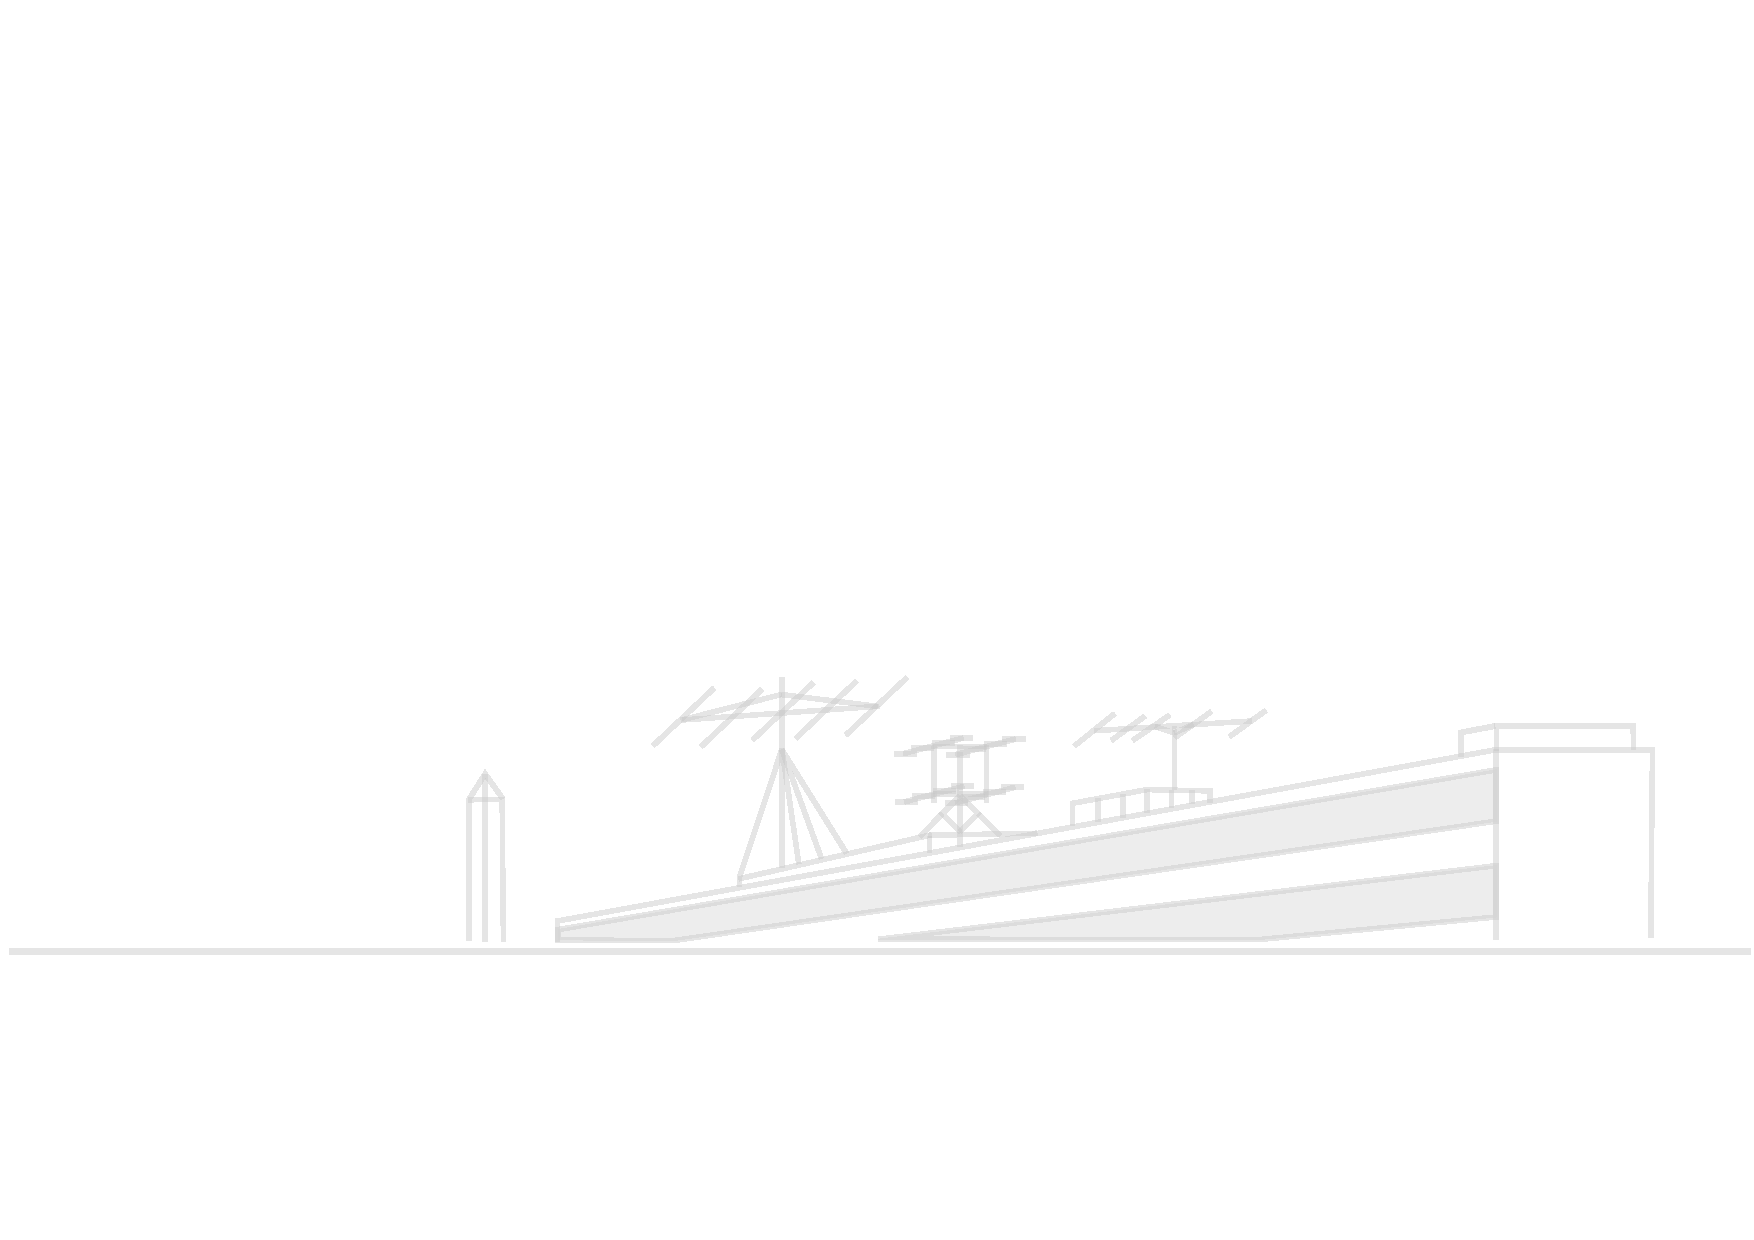
\includegraphics[width=17.8cm]{texdata/dk0tu_rooftop_background.pdf}
}

% Foliennummer einfügen
\setbeamertemplate{footline}[frame number]
%\setbeamertemplate{footline}{}

% Ändere das Zeichen vor jedem item
%\setbeamertemplate{itemize item}{\color{craneorange}$\blacktriangleright$}
%\setbeamertemplate{itemize subitem}{\color{craneorange}$\triangleright$}
%\setbeamertemplate{itemize subsubitem}{\color{craneorange}$\blacktriangleright$}

% Ändert die Blöcke 
\setbeamertemplate{blocks}[rounded][shadow=true]
% default | rounded [shadow=true|false]

%
% Eigene Kommandos
%

% Hack to get natbib and beamer working together. "The beamer user guide suggests
% that only the manual bibliography entry approach is supported"
% on some system it works out of the box, sometimes you need the hack :-(
% so check it --dl7bst
\ifdefined\newblock
    \relax
\else
    \newcommand{\newblock}{}
\fi

% \includedia command to generate png out of a dia file
% NEEDS installed dia and pdflatex option --shell-escape
\newcommand{\includedia}[1]{
    \immediate\write18{/usr/bin/dia #1.dia -e #1_diatmp.png -t png}
}

% RICHIG GROSSER FONT!
\newfont{\bigfont}{cmr10 at 144pt}
\newfont{\smallfont}{cmr10 at 8pt}

% Römische Ziffern
\makeatletter
\newcommand{\rmnum}[1]{\romannumeral #1}
\newcommand{\Rmnum}[1]{\expandafter\@slowromancap\romannumeral #1@}
\makeatother

% Schwarze Überschrift
%\setbeamercolor{frametitle}{fg=black}
%\setbeamercolor{title}{fg=black}

% Item- und Box-Farben
\definecolor{deepBlue}{HTML}{000066}
\setbeamercolor{itemize item}{fg=deepBlue}
\setbeamercolor{itemize subitem}{fg=deepBlue}
\setbeamercolor{description item}{fg=deepBlue}
\setbeamercolor{block title}{fg=deepBlue!100, bg=blue!15}
\setbeamercolor{block body}{fg=black, bg=blue!5}
\setbeamercolor{block title alerted}{fg=deepBlue, bg=red!75}
\setbeamercolor{block body alerted}{fg=black, bg=red!15}
\setbeamercolor*{block title example}{fg=blue!50, bg=blue!10}
\setbeamercolor*{block body example}{fg= blue, bg=blue!5}

%\setbeamercolor{section in head/foot}{parent=palette primary}
%\setbeamercolor{subsection in head/foot}{parent=palette secondary}
%\setbeamercolor{sidebar}{fg=darkblue,bg=yellow!90!orange}
%\setbeamercolor{title in sidebar}{fg=darkblue}
%\setbeamercolor{author in sidebar}{fg=darkblue}
%\setbeamercolor{section in sidebar}{fg=darkblue!10!black}
%\setbeamercolor{subsection in sidebar}{fg=darkblue!50!black}

% Titlepage Infos
\title{AFu-Kurs nach DJ4UF}
\author[DKØTU]{DKØTU\\ \footnotesize{Amateurfunkgruppe der TU Berlin}}
\institute[DKØTU]{\url{http://www.dk0tu.de} }

% PDF-Eigenschaften
\subject{DK0TU-Amateurfunkkurs nach DJ4UF}
\keywords{Amateurfunk Kurs HAM Radio Course CC-BY-NC-SA OpenSource TU Berlin DK0TU}

\subtitle{Technik Klasse E 13: \\
  Transistor \& Verstärker \\[2em]}
\date{Stand 28.11.2016}
 \begin{document}

\begin{frame}
    \titlepage
    \vfill
    \begin{center}
        \ccbyncsaeu\\
        {\tiny This work is licensed under the \em{Creative Commons Attribution-NonCommercial-ShareAlike 3.0 License}.}\\[0.5ex]
         \tiny Amateurfunkgruppe der Technische Universität Berlin (AfuTUB), DKØTU
         %\includegraphics[scale=0.5]{img/DK0TU_Logo.pdf}
    \end{center}
\end{frame}


%fixme Referenzen/Fußnoten-Systematik vereinheitlichen

\section*{Einleitung}
\begin{frame}
  \frametitle{Einleitung}
  Wir erinnern uns $\rightarrow$ Video aus \texttt{E12}\\[1.5em]
  Was macht ein Transistor?
  \only<2>{\begin{itemize}
    \item verstärken (analog)
    \item schalten (digital)
  \end{itemize}
  }
\end{frame}

\begin{frame}
  \frametitle{Transistoren}
  \begin{figure}
    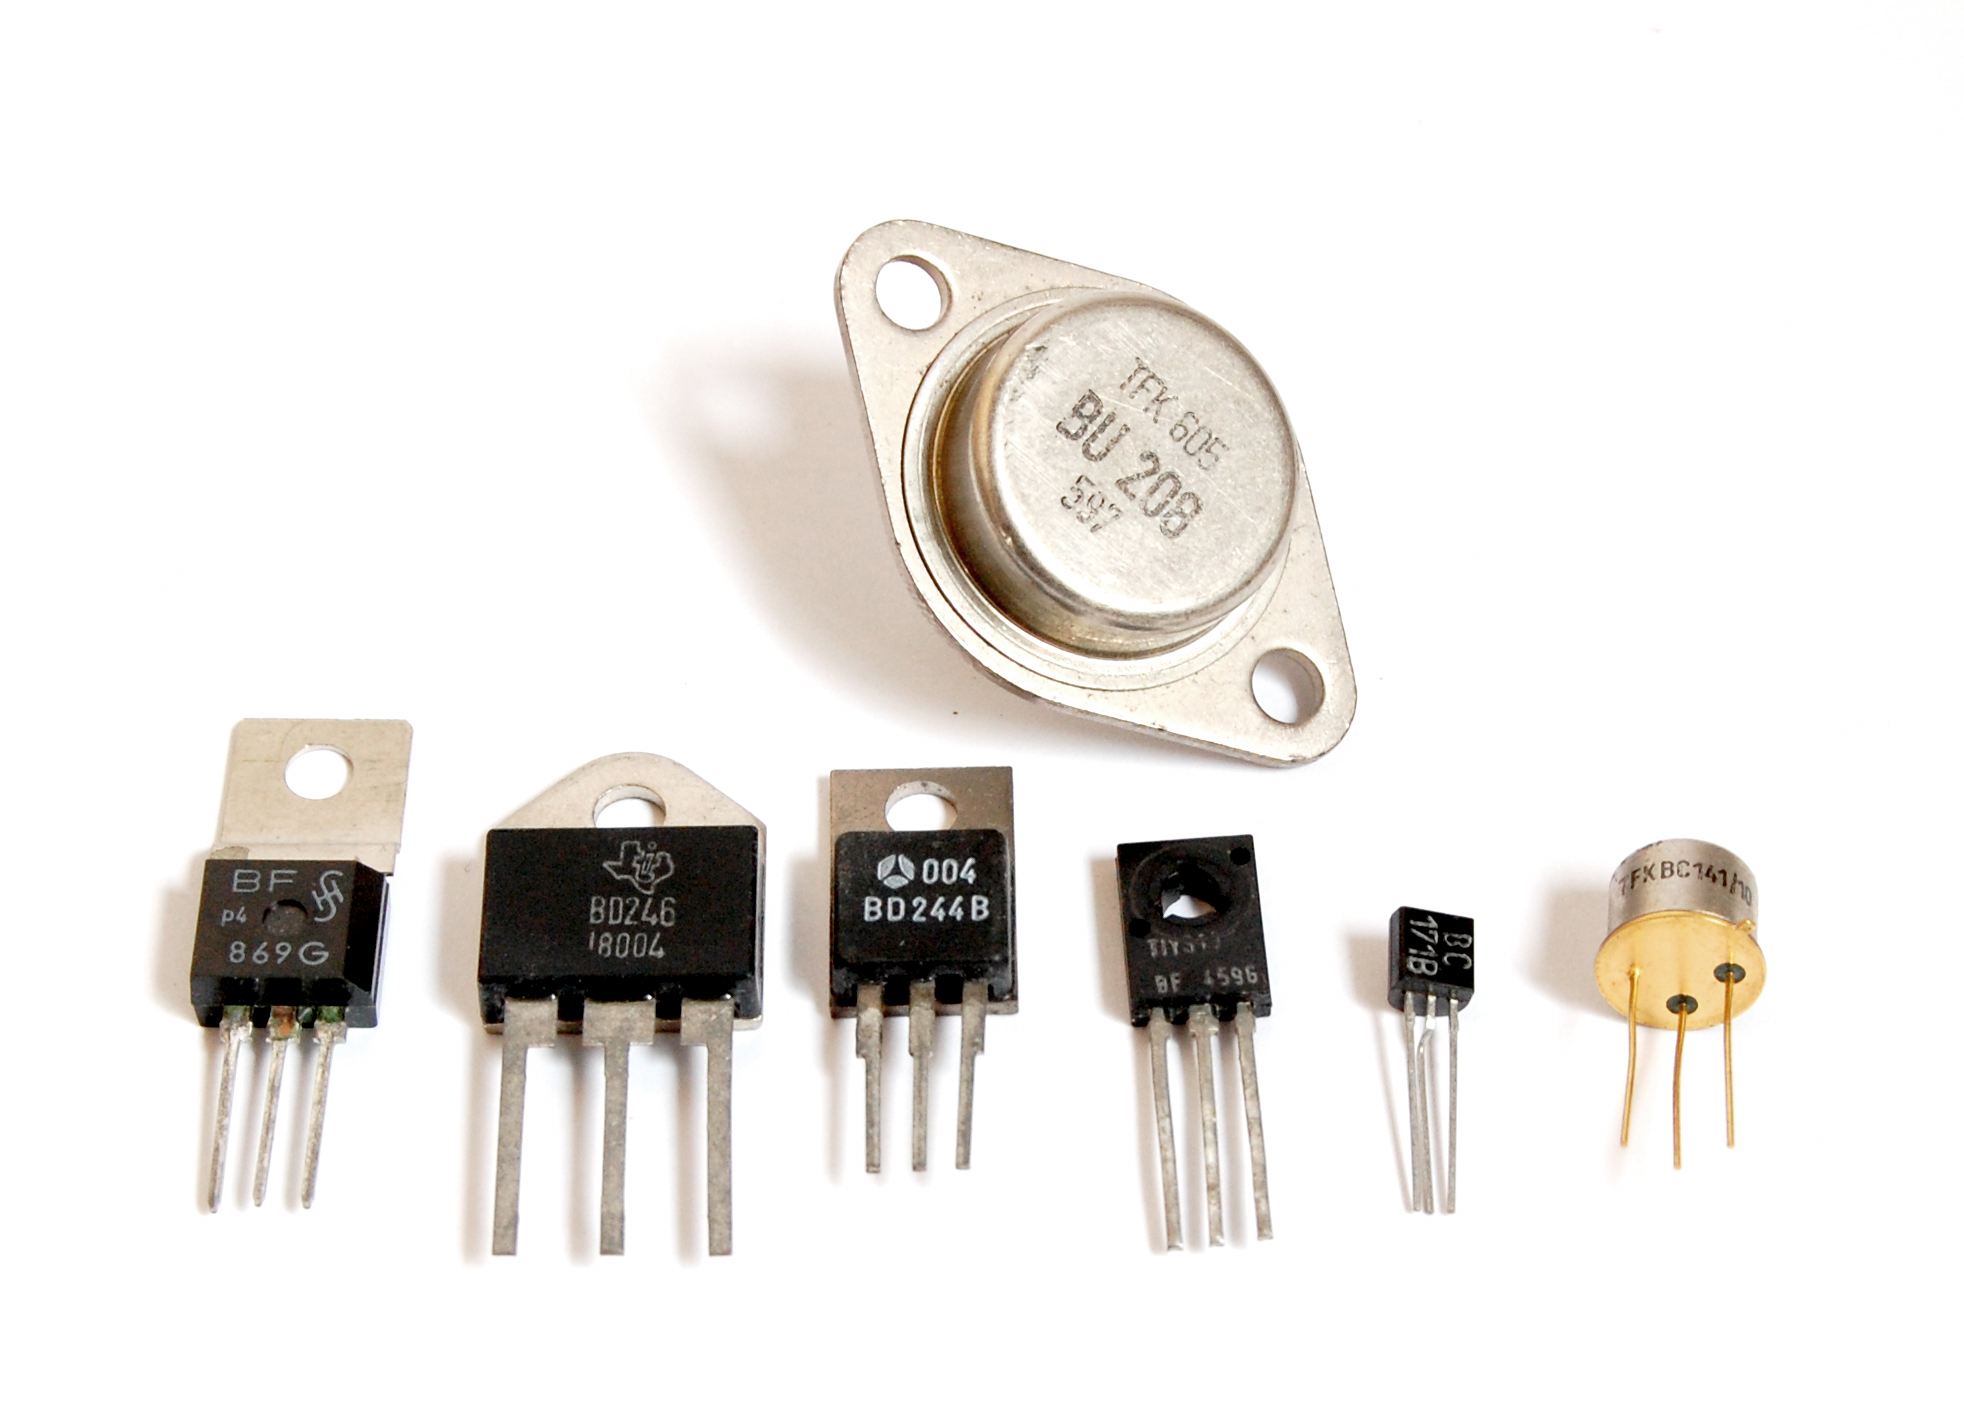
\includegraphics[width=\textwidth,height=.65\textheight,keepaspectratio]{e13/Transistors-white.jpg}
    \attribcaption{Verschiedene Transistor-Bauformen}{Benedikt.Seidl}{https://commons.wikimedia.org/wiki/File:Transistors-white.jpg}{\ccpd}
  \end{figure}
\end{frame}

\section*{Bipolarer Transistor}
\begin{frame}
  \frametitle{Bipolarer Transistor}
  \begin{minipage}{0.4\textwidth}
    \begin{figure}
      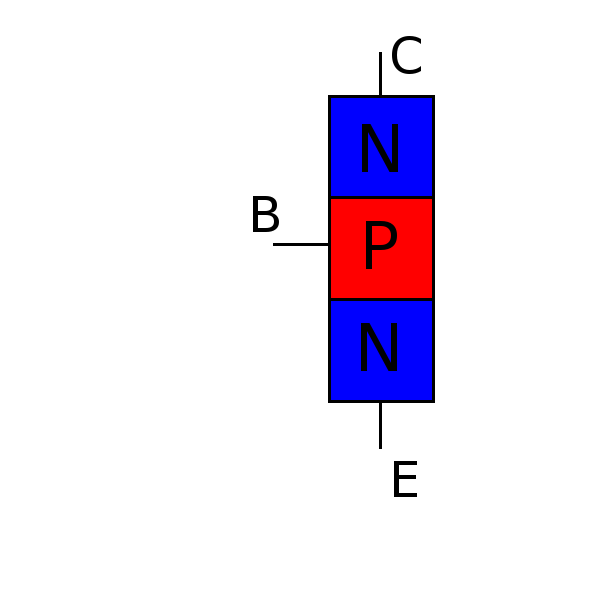
\includegraphics[width=\textwidth,height=.4\textheight,keepaspectratio]{e13/NPN_hlb.png}\\
      \caption{Schichten eines \hbox{NPN-Transistors}}
    \end{figure}
  \end{minipage}
  \hspace{0.5cm}
  \begin{minipage}{0.4\textwidth}
    \begin{figure}
      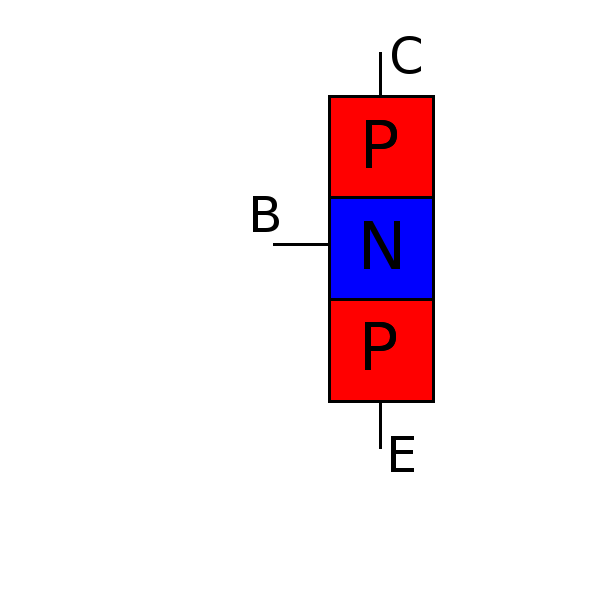
\includegraphics[width=\textwidth,height=.4\textheight,keepaspectratio]{e13/PNP_hlb.png}\\
      \caption{Schichten eines \hbox{PNP-Transistors}}
    \end{figure}
  \end{minipage}
  \vspace{0.5cm}
  \begin{center}
    \begin{itemize}
      \item Transistoren bestehen aus drei Halbleiterschichten
      \item Anschlüsse: Basis (B), Kollektor (C), Emitter (E)
    \end{itemize}

  \end{center}
\end{frame}

\begin{frame}
  \frametitle{Ersatzschaltbild}

  \begin{minipage}{0.4\textwidth}
    \begin{figure}
      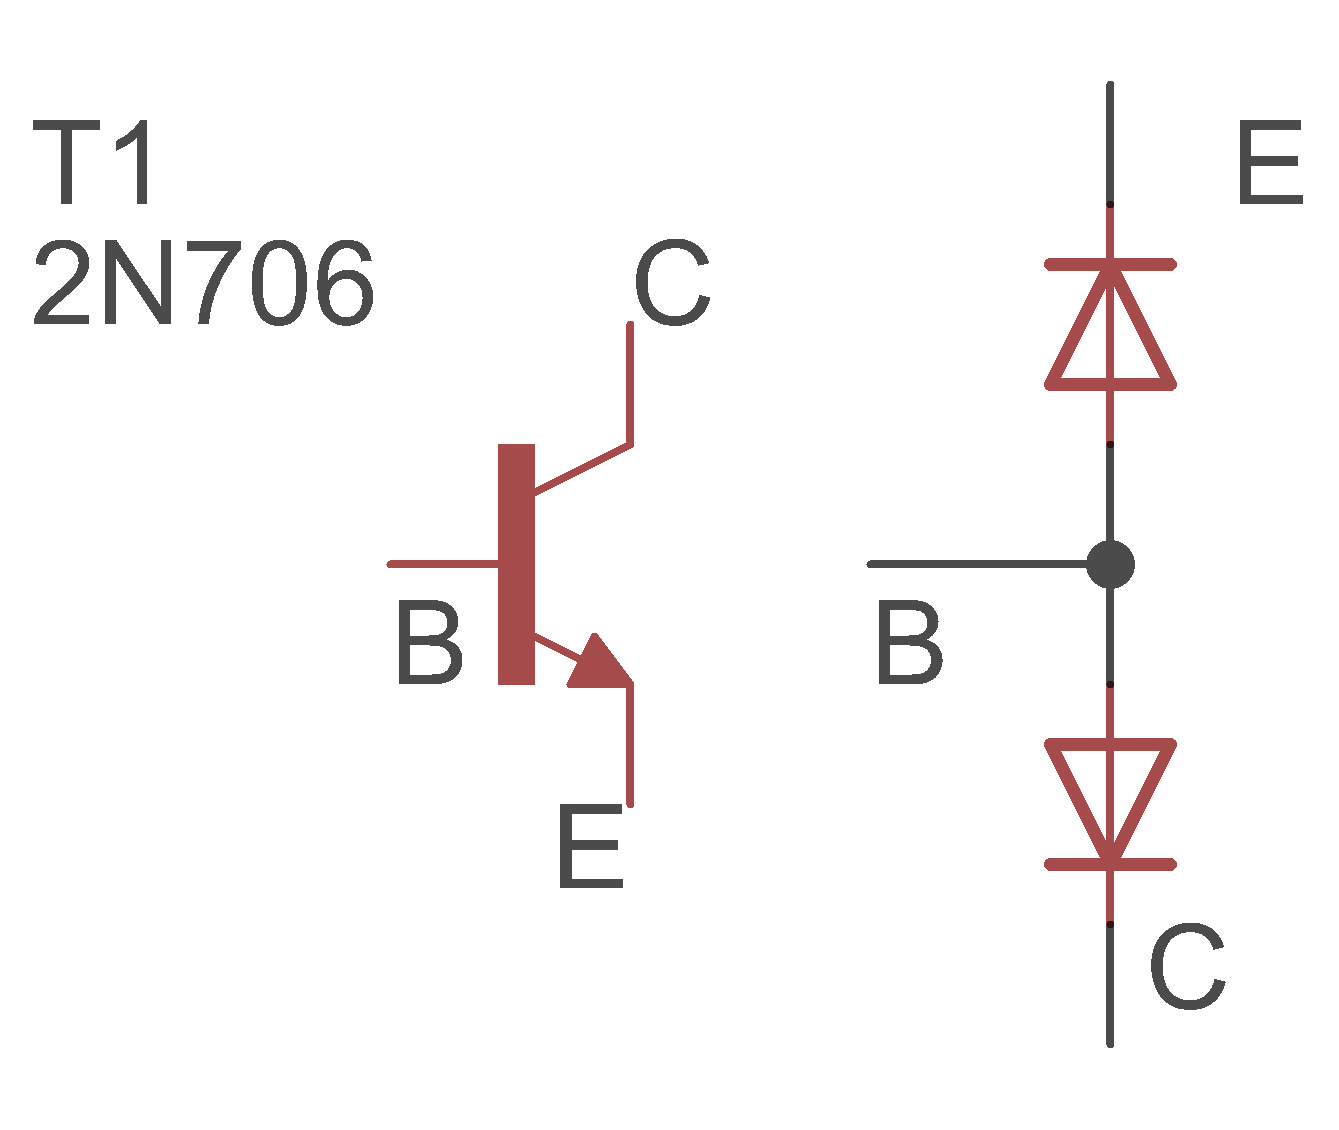
\includegraphics[width=\textwidth,height=.4\textheight,keepaspectratio]{e13/NPN_esb.png}
      \caption{ESB eines \hbox{NPN-Transistors}}
    \end{figure}
  \end{minipage}
  \hspace{0.5cm}
  \begin{minipage}{0.4\textwidth}
    \begin{figure}
      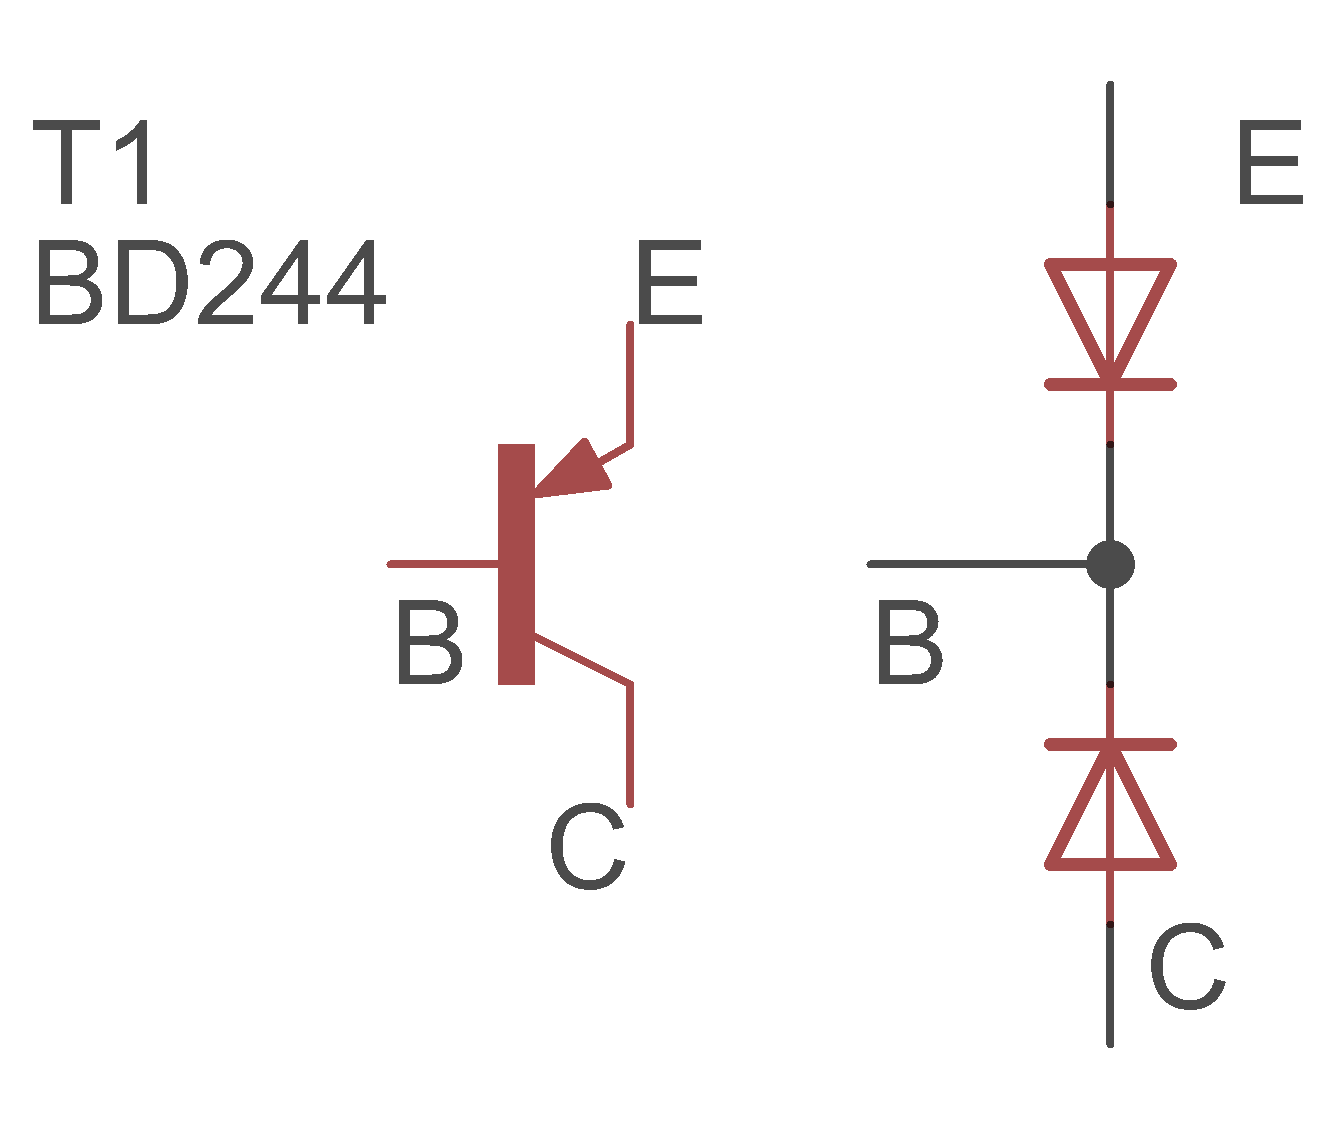
\includegraphics[width=\textwidth,height=.4\textheight,keepaspectratio]{e13/PNP_esb.png}
      \caption{ESB eines \hbox{PNP-Transistors}}
    \end{figure}
  \end{minipage}

  \begin{center}
    \begin{block}{Funktionsweise}
      Der Basisstrom steuert den Kollektorstrom
      $$I_{CE} = I_{BE} \cdot \beta$$
    \end{block}
  \end{center}
\end{frame}

\begin{frame}
  \frametitle{Bipolartransistor Verständnis}
  \begin{minipage}{0.55\textwidth}
    \begin{center}
      \only<1>{
      \begin{figure}
        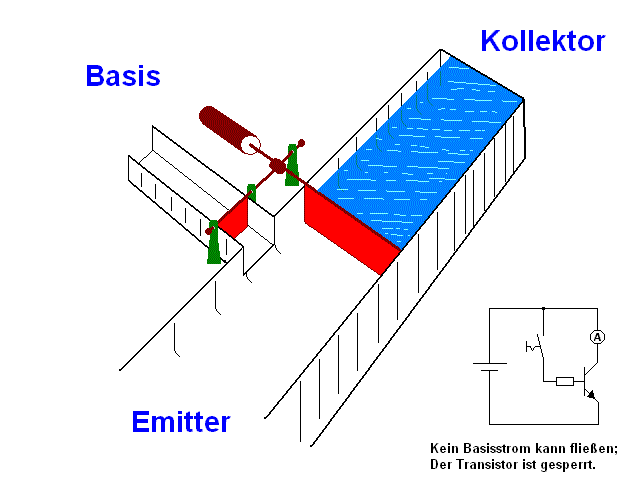
\includegraphics[scale=0.3]{e13/Transistor_animation1.png}
        \attribcaption{Animation eines alternativen Transistormodells (geschlossen)}{Stefan Riepl}{https://commons.wikimedia.org/wiki/File:Transistor_animation.gif}{\ccbysa}
      \end{figure}
      }
      \only<2>{
      \begin{figure}
        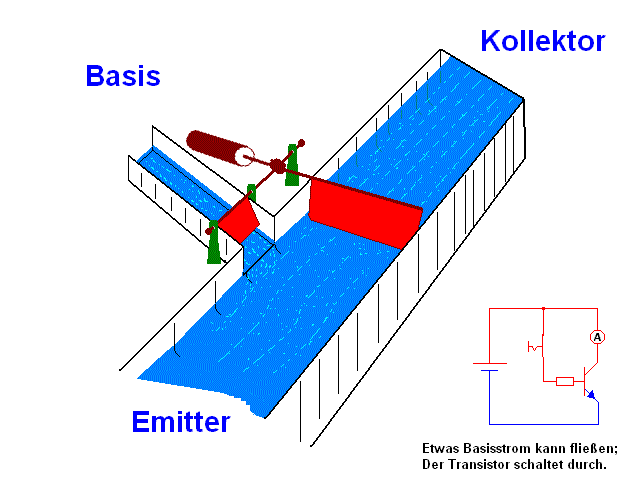
\includegraphics[scale=0.3]{e13/Transistor_animation2.png}
        \attribcaption{Animation eines alternativen Transistormodells (offen)}{Stefan Riepl}{https://commons.wikimedia.org/wiki/File:Transistor_animation.gif}{\ccbysa}
      \end{figure}
      }
    \end{center}
  \end{minipage}
  \begin{minipage}{0.4\textwidth}
    \begin{center}
      \begin{block}{Funktionsweise}
        Der Basisstrom steuert den Kollektorstrom
        $$I_{CE} = I_{BE} \cdot \beta$$
        $\beta = $ Verstärkungsfaktor \\ (Modellabhängig $\beta = 10-900$)
      \end{block}
    \end{center}
  \end{minipage}
\end{frame}


\begin{frame}
  \frametitle{Ersatzschaltbild}

  \begin{minipage}{0.4\textwidth}
    \begin{figure}
      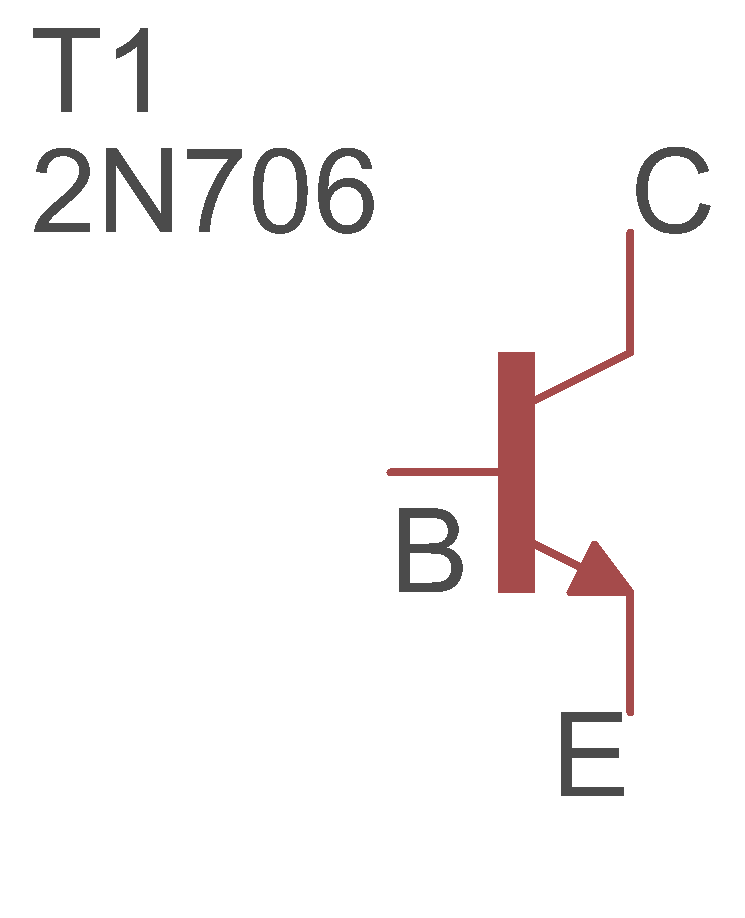
\includegraphics[width=\textwidth,height=.4\textheight,keepaspectratio]{e13/NPN.png}
      \caption{NPN Transistor -- \textbf{N}icht \textbf{P}feil \textbf{N}ach Platte}
    \end{figure}
  \end{minipage}
  \hspace{0.5cm}
  \begin{minipage}{0.4\textwidth}
    \begin{figure}
      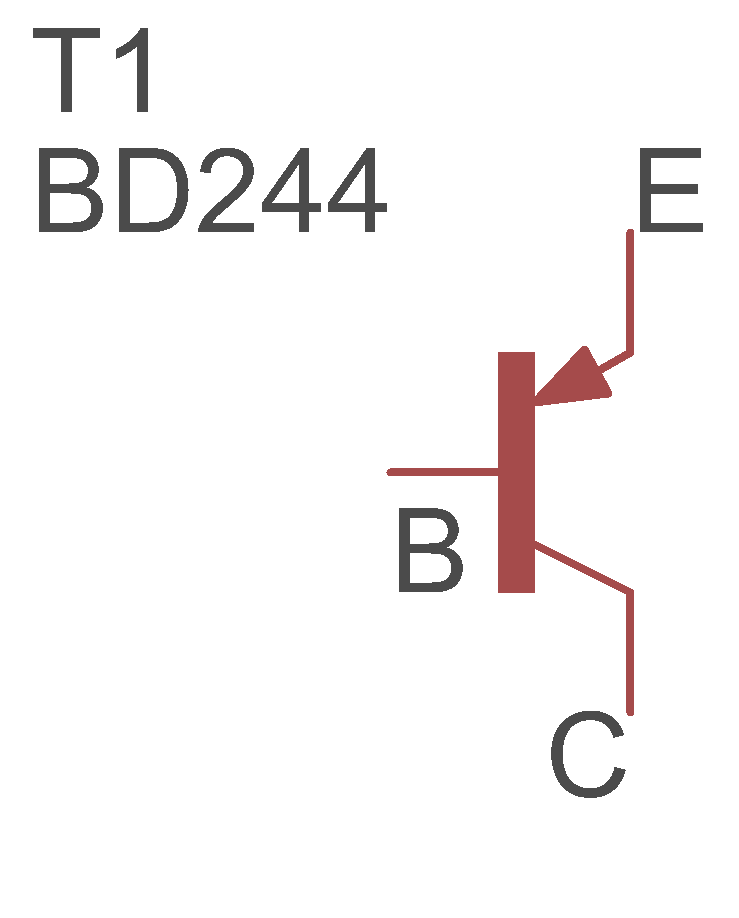
\includegraphics[width=\textwidth,height=.4\textheight,keepaspectratio]{e13/PNP.png}
      \caption{PNP Transistor -- \textbf{P}feil \textbf{N}ach \textbf{P}latte}
    \end{figure}
  \end{minipage}

  \begin{center}
    \begin{block}{Funktionsweise}
      NPN Transistor braucht $ U_{BE}=+0.7V$ zum Schalten\\
      PNP Transistor braucht $ U_{BE}=-0.7V$ zum Schalten\\
      Beide sind Stromgesteuert $I_{CE} = I_{BE} \cdot \beta$
    \end{block}
  \end{center}
\end{frame}

\section*{Feldeffekt Transistor (FET)}
\begin{frame}
  \frametitle{Metall Oxid Semiconductor Feldeffekt Transistor (MOSFET)}
  \begin{center}
    \begin{figure}
      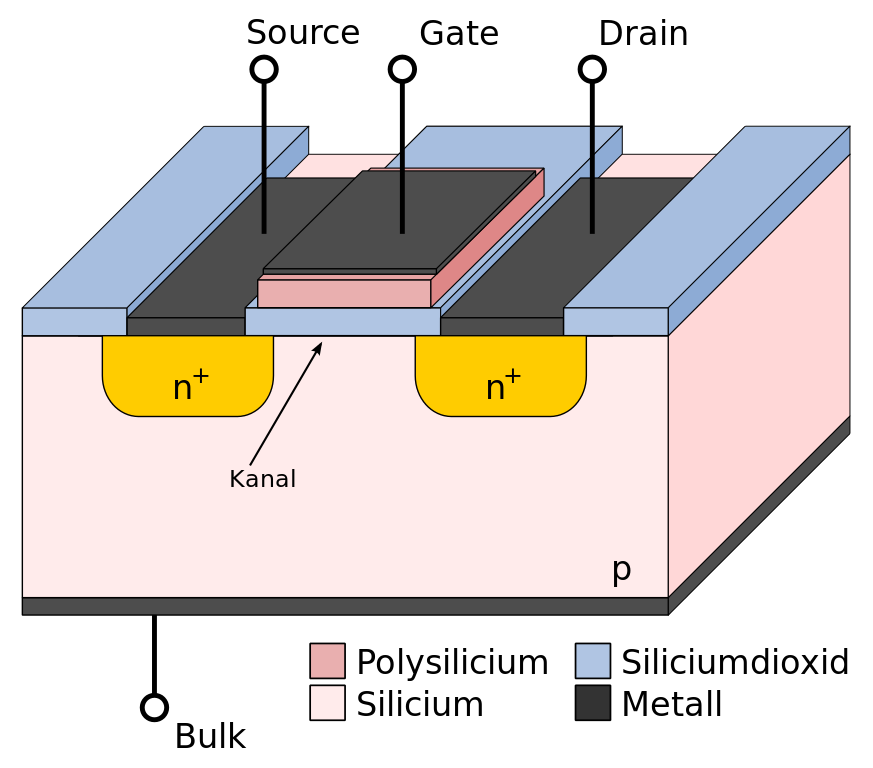
\includegraphics[width=\textwidth,height=.65\textheight,keepaspectratio]{e13/N-Kanal-MOSFET.png}
      \attribcaption{MOSFET in Planartechnologie}{PNG-Version: Markus A. Hennig, SVG-Umsetzung: Cepheiden}{https://commons.wikimedia.org/wiki/File:N-Kanal-MOSFET_(Schema).svg}{\ccbysa}
    \end{figure}
  \end{center}
\end{frame}

\begin{frame}
  \frametitle{Metall Oxid Semiconductor Feldeffekt Transistor (MOSFET)}
  \begin{center}
    \begin{figure}
      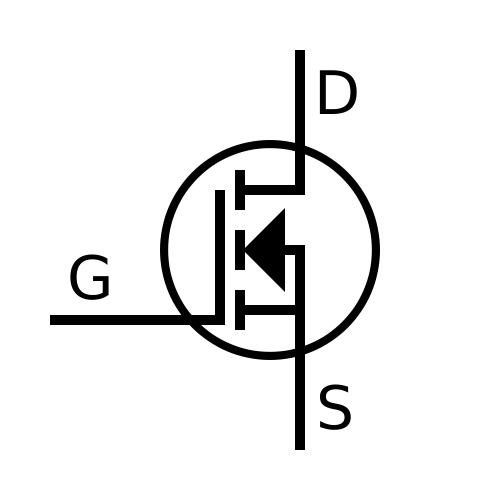
\includegraphics[width=\textwidth,height=.4\textheight,keepaspectratio]{e13/N-Ch_Enh_Labelled.png}
      \caption{N-Kanal beschriftet}
    \end{figure}
    \begin{block}{Funktionsweise}
      \begin{itemize}
        \item Gate steuert Kanalbreite durch Spannung $U_{GS}$
        \item Je größer $U_{GS}$ desto größer $I_{DS}$, da $R_{DS}$ kleiner wird
      \end{itemize}
    \end{block}
  \end{center}
\end{frame}

\begin{frame}
  \frametitle{Feldeffekt Transistor (FET)}
  \begin{center}
    \begin{figure}
      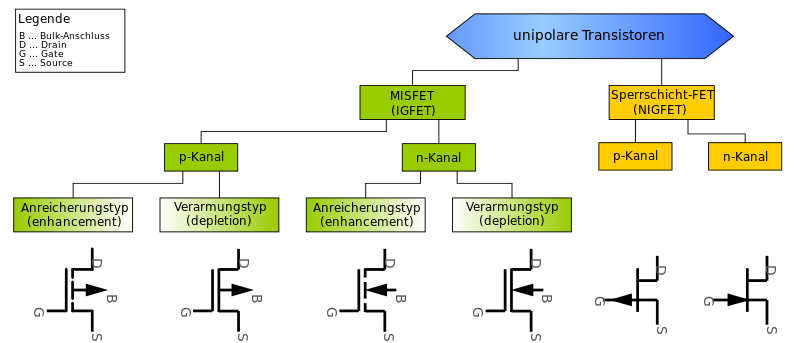
\includegraphics[width=\textwidth,height=.65\textheight,keepaspectratio]{e13/FET-overview.png}
      \attribcaption{Übersicht über FETs}{Cepheiden}{https://commons.wikimedia.org/wiki/File:FET-Typen_(mit_Schaltbildern).svg}{\ccpd}
    \end{figure}
  \end{center}
\end{frame}

\section{Verstärker}
\begin{frame}
  \frametitle{Verstärker}
  \begin{center}
    \begin{block}{Definition eines Verstärkers nach Captain Obvious}
      \begin{Large}
        Es ist nur dann eine Verstärkung, wenn die Leistung am Ausgang größer ist, als die am Eingang
      \end{Large}
    \end{block}
  \end{center}
\end{frame}

\section*{Operations\-verstärker}
\begin{frame}
  \frametitle{Operationsverstärker}
  \begin{minipage}{0.4\textwidth}
    \begin{figure}
      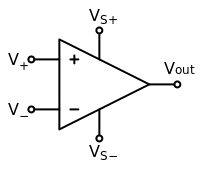
\includegraphics[width=\textwidth,height=.4\textheight,keepaspectratio]{e13/OPV.png}
      \attribcaption{OPV nach ANSI}{Omegatron}{https://commons.wikimedia.org/wiki/File:Op-amp_symbol.svg}{\ccbysa}
    \end{figure}
  \end{minipage}
  \hspace{0.5cm}
  \begin{minipage}{0.4\textwidth}
    \begin{figure}
      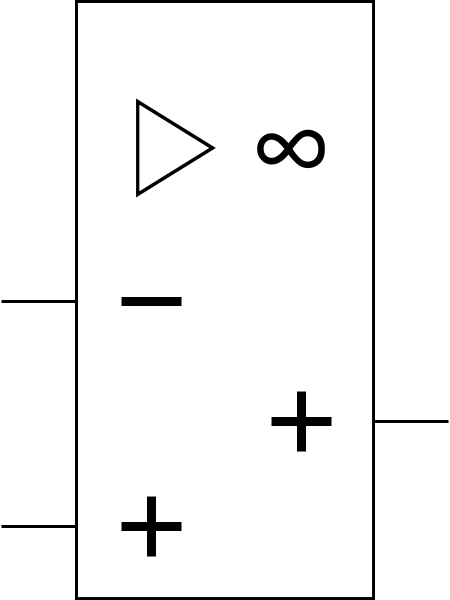
\includegraphics[width=\textwidth,height=.4\textheight,keepaspectratio]{e13/OPV-ger.png}
      \attribcaption{OPV nach DIN}{Daniel Braun}{https://commons.wikimedia.org/wiki/File:Normsymbol_OPV.svg}{\ccpd}
    \end{figure}
  \end{minipage}
  \begin{center}
    \begin{itemize}
      \item OPV  sind gleichspannungsgekoppelte elektronische Verstärker
      \item sehr hohe (idealerweise unendliche) Verstärkung
      \item Anschlüsse für Versorgungsspannung
      \item die Grundschaltung ist ein Differenzverstärker
      \item diverse Schaltungsarten für unterschiedliche Funktionsweisen möglich
    \end{itemize}
  \end{center}
\end{frame}

\begin{frame}
  \frametitle{Operationsverstärker}
  \begin{center}
    \begin{figure}
      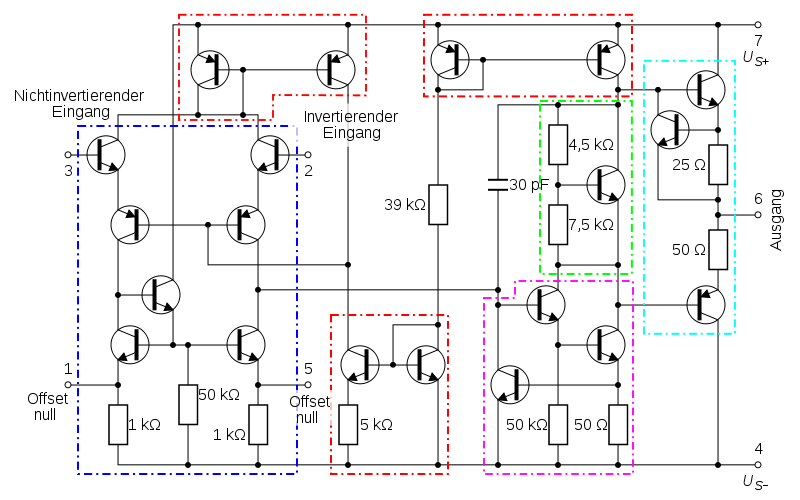
\includegraphics[width=\textwidth,height=.65\textheight,keepaspectratio]{e13/OPV-intern.png}
      \attribcaption{Innerer Aufbau eines OPVs}{Daniel Braun derivative work: Cepheiden}{https://commons.wikimedia.org/wiki/File:OpAmpTransistorLevel_Colored_DE.svg}{\ccbysa}
    \end{figure}
  \end{center}
\end{frame}

\section*{Integierte Schaltung}
\begin{frame}
  \frametitle{Integierte Schaltung}
  Heutzutage komplexe Schaltungen auf einem Halbleiterkristall
  \begin{minipage}{0.3\textwidth}
    \begin{figure}
      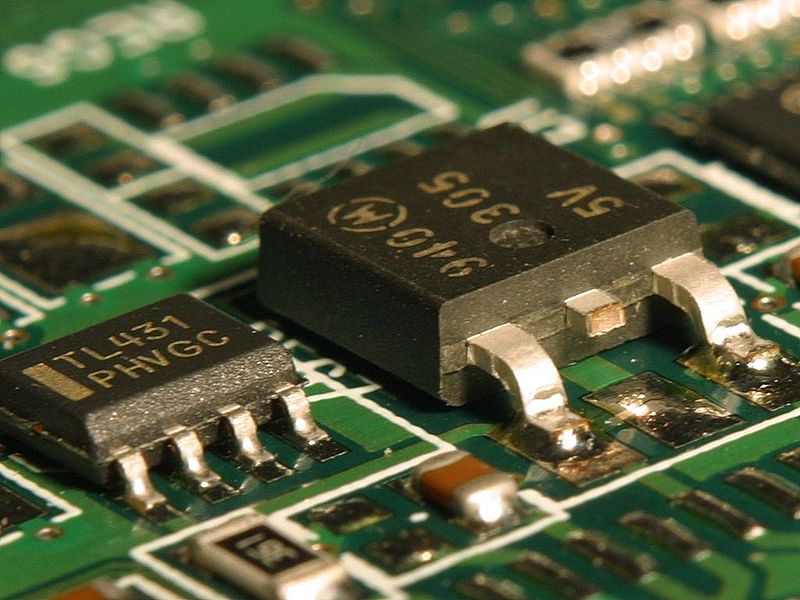
\includegraphics[width=\textwidth,height=.6\textheight,keepaspectratio]{e13/IC.jpg}
      \attribcaption{IC auf einer Platine}{Luestling}{https://commons.wikimedia.org/wiki/File:Chips_3_bg_102602.jpg}{\ccpd}
    \end{figure}
  \end{minipage}
  \hspace{0.5cm}
  \begin{minipage}{0.5\textwidth}
    \vspace{0.5cm}
    \begin{center}
      \begin{figure}
        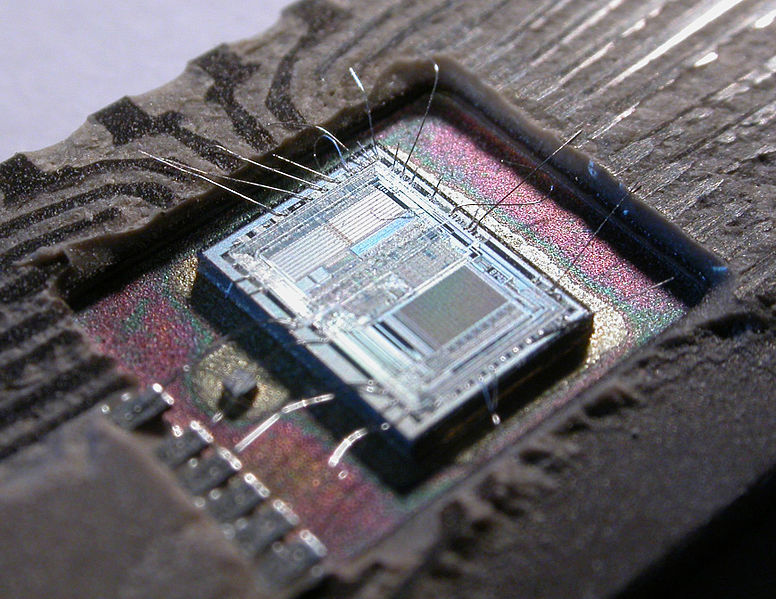
\includegraphics[width=\textwidth,height=.6\textheight,keepaspectratio]{e13/IC2.jpg}
        \attribcaption{Offener IC}{Ioan Sameli}{https://commons.wikimedia.org/wiki/File:Intel_8742_153056995.jpg}{\ccbysa}
      \end{figure}
    \end{center}
  \end{minipage}
\end{frame}

\section*{Die Röhre}
\begin{frame}
  \frametitle{Die Röhre}
  \begin{minipage}{0.3\textwidth}
    \begin{figure}
      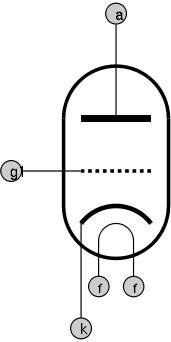
\includegraphics[width=\textwidth,height=.5\textheight,keepaspectratio]{e13/ERohre.png}
      \attribcaption{Symbol einer Triode}{RokerHRO, geändert von Fgli}{https://commons.wikimedia.org/wiki/File:Triode-Symbol_de.svg}{\ccpd}
    \end{figure}
  \end{minipage}
  \hspace{0.5cm}
  \begin{minipage}{0.5\textwidth}
    \begin{small}
      \begin{itemize}
        \item Heizung löst Elektronen aus Kathode
        \item Elektronen werden Richtung Anode beschleunigt
        \item Gitter verändert elektrisches Feld
        \item Gitterspannung steuert Anodenstrom
      \end{itemize}
    \end{small}
    \begin{center}
      \begin{figure}
        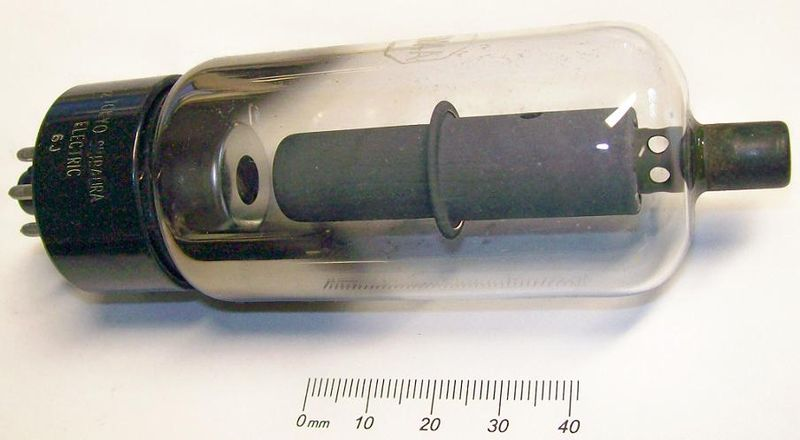
\includegraphics[width=\textwidth,height=.3\textheight,keepaspectratio]{e13/Triode.jpg}
        \attribcaption{Triode aus alten Fabfernsehern}{Ulfbastel}{https://commons.wikimedia.org/wiki/File:Strahltriode.jpg}{\ccby}
      \end{figure}
    \end{center}
  \end{minipage}
\end{frame}

\appendix
\section*{Referenzen}
\begin{frame}
  \frametitle{Referenzen/Links}

  \footnotesize
  \begin{itemize}
    \item Moltrecht E 13 : \\
      \url{https://www.darc.de/der-club/referate/ajw/lehrgang-te/e13/}
    \item Elektronik Kompendium:
      \url{http://www.elektronik-kompendium.de/sites/bau/index.htm}
  \end{itemize}

\end{frame}


% Hier könnte noch eine Kontaktfolie stehen

\end{document}

